\chapter{State estimation for legged robots: a literature review}
%
The field of state estimation for autonomous systems is at the frontier between many fields including automation, probability theory, non linear estimation etc.
The general aim is to design and implement computationally tractable algorithms using noisy causal sensor measurements that can be embedded in feedback controlled systems.
With the advent of digital computers and the theoretical breakthroughs of Kalman \cite{kalman1960new} among others, a vast family of observers has been developed 
\cite{fujii2013extended, wan2001unscented} [cite Information filter]. Applications range the full scope of autonomous systems from spacecraft guidance \cite{mcgee1985discovery} 
to autonomous underwater vehicle navigation \cite{leonard2016autonomous}. Each application has its own specific sets of requirements, depending on the physical
nature of the system and its environment, available sensors and embedded computation power. Legged robots in particular require a high frequency (kHz) 
and low latency estimates owing to the inherent instability of the dynamical system. Moreover they interact with the environment through 
intermittent contacts to move around which require to plan in advance the motion using Model Predictive Control (MPC). These tight requirements 
have given birth to a wealth of research works are now commonly used in commercial products \cite{hutter2016anymal}.

We will focus our review on works applying state estimation theory on legged robots, which include mainly quadrupeds and humanoid robots. The first part will 
be centered around proprioceptive estimation of the robot main body. We will then examine the estimation of centroidal quantities. The use of exteroceptive sensors
to obtain information from the robot environment will then be described. Finally, we will see that a new class of optimization based estimator is a promising alternative
to filtering based methods.

\section{Definitions}
\label{sec:def}
Let's first introduce terms and key concepts that are commonly used in the legged robot estimation literature.

\textit{Legged robot} are poly-articulated systems that use a set end effectors (commonly referred to as feet whatever their nature) to move their main body
by pushing on its environment. The kinematic chain of the robot is modeled as a graph composed of fixed shape segments (aka. links) 
linked together by articulations (aka. joints). Joints come in various forms (revolute, prismatic, ball...) and can be actuated or not.
The \textit{base} refers to a reference frame rigidly attached to the main body of the robot (often the trunk for quadrupeds and the pelvis for humanoids). 
We are most often interested in the estimation of the position, velocity and orientation of this frame with regard to an inertial \textit{world} frame, which is called the \textit{base state}. 
This estimation is the main focus in most of legged robot estimation literature. In fact, knowing the base base and other quantities directly measurable (such as joint angles), 
and assuming a perfect robot kinematic model, the state of any part of the multibody system can be recovered using forward kinematics. Rigid body algorithms
\cite{featherstone2014rigid} provide methods to efficiently compute the center of mass, linear and angular momentum of the multi body systems. These computations
are again based on the robot kinematic model as well as the segments inertia, which we together call the $kinodynamic$ robot model. This model is often 
found in urdf files (Unified Robot Description Format) which are generated via CAD models.

The \textit{centroidal state} refer to the center of mass, angular momentum and their derivatives. The center 
of mass (barycenter of the robot segment masses) is a virtual point that is the main control variable for locomotion. 
%Centroidal estimators fuse the robot kinematic model, which is often assumed to be biased, with various dynamical models of the system. 

\textit{Proprioceptive} sensors measure values about the internal state the robot. For legged robots, they include joint encoders, strain gauges measuring 
either joint torques or end effector torques, dedicated feet contact sensors and Inertial Measurement Units (IMUs). These sensors do not directly provide information
about the external robot environment and can therefore only be used to compute a drifting pose of the robot, the odometry \footnote{The status of an IMU is debatable
since an accelerometer measures the external gravity vectors which can be used to infer an approximate but non drifting orientation. It is however often considered 
a proprioceptive sensor in the legged robot literature \cite{rotella2018unsupervised,scona2017direct,yang2019state,lin2021deep}}. 

\textit{Exteroceptive} sensors (cameras, depth cameras, LIDARs...) provide information about the environment of the robot.  
They are needed to obtain non drifting estimates of the robot pose. 
They are used either to localize with respect to a map or to build a representation of the environment online, that the robot can use to plan contact for instance. 

% TOO OPINIONATED RIGHT OF THE BAT -> need to present more the logic of the chapter
% These problems are often compartmentalized in the literature. Separate estimators are developed tackling each problem and communicate their results as priors for the others. 
% This approach often makes the problem more computationally tractable and may reduce the software complexity by dividing code bases. However, from the estimation
% point of view this approach may result in sub-optimal, even inconsistent estimators by neglecting cross correlations between variables. In particular,
% coupling odometry sources with environment reconstruction has been widely explored in the SLAM literature, which has shifted to estimators based on batch optimization.
% This technique has recently been making its way into the legged robot literature.



\begin{figure}
    \centering
    \label{fig:solo_frames}
    \centering
    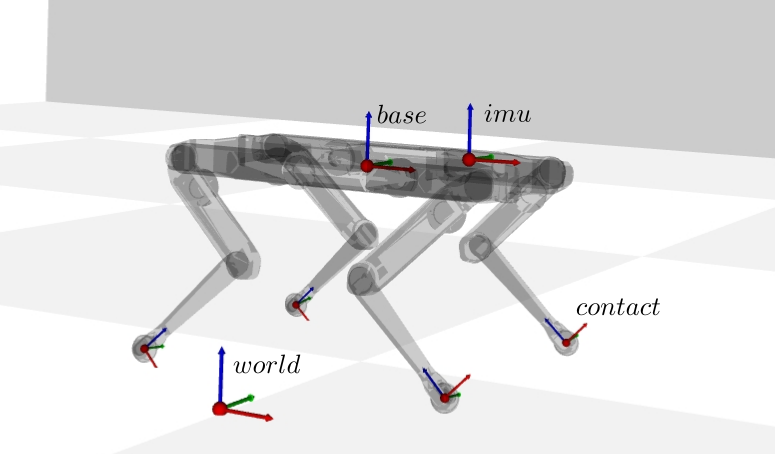
\includegraphics[width=0.6\textwidth]{figures/solo_frames.pdf}
    \caption{Solo 12 \cite{grimminger2020open} important reference frames}
\end{figure}
    

%%%%%%%%%%
\section{Proprioceptive base estimation}


We refer to proprioceptive base estimation for any state observer purely relying on proprioceptive sensors to estimate base frame states. 
The goal is then to design observers fusing IMU, kinematics and possibly strain gauges measurements to obtain an odometry and orientation of 
the robot with respect to the gravity vector. The robot is akin to a blindfolded animal that has to balance and perform locomotion using 
only its inner ear, kinesthesis and sense of touch. \cite{bloesch2013state,rotella2014state} showed through an observability analysis 
that the absolute velocity, pitch and roll angles as well as IMU biases are observable using only IMU and kinematic measurements when at 
least one contact is kept with the ground.

The robotician has to make many design choices when building such a system. Those choices mainly include the way kinematic information is used in the system, 
the nature of the filter used (tightly-coupled vs loosely-coupled), how to detect stable contacts and whether extra sensors or more complex modeling need 
to be used to mitigate model errors.
 

\subsection{Kinematic information}
Legged robots move by interacting with their environment through intermittent contacts.
Once a stable contact (no slipping/tipping) is detected, the relative pose and velocity of the base with respect to the end effector in contact 
can be computed through forward kinematics. Integrated over time, the relative displacement of the base of the robot can be inferred, a computation 
often referred to as \textit{leg odometry} (by analogy with wheel odometry). This computation takes about 1 microsecond thanks to libraries such as \cite{carpentier2019pinocchio, hereid2017frost}. It uses
readings from the joints encoders as well as the robot kinematic model. In systems with actuator reduction steps, encoders are usually placed before the reduction step 
which are very accurate (... for solo \cite{grimminger2020open}). Joint velocities are often less precise since they are generally computed from numerical differentiation \cite{rotella2016imu}. 
The main sources of uncertainty usually comes from inaccuracies in the parameters of the kinematic models such as approximate segment lengths, segments flexibilities \cite{vigne2018estimation}, 
joint backlash \cite{fallon2014drift} and flexibilities \cite{koolen2016design}. 
Bloesch \cite{bloesch2018technical} classifies kinematic measurement models in three categories that define the structure of this section. 
Those measurement models are summarized in \figRef{fig:kin_models}.


\textit{Feet matching} is the earliest example of leg odometry to be used in the leg robotics literature. Pioneered by \cite{roston1991dead} 
\footnote{An earlier example might exist in \cite{waldron1986adaptive} even though the technical report is unclear about the method they used: 
"Leg-position feedback is used from legs in support phase for the purpose of correcting for gyro and integration drift in the inertial reference system."},
multiple feet matching provides a relative 6D pose between moments during which at least three feet are in stable contact with the ground.
For point-feet robots (such as most quadrupeds), the problem is an instance of the orthogonal Procrustes problem.
Follow up works adapted the method to smaller hexapods \cite{lin2005leg} and began to fuse it with other sensors such as GPS \cite{gassmann2005localization, cobano2008location} 
and most importantly IMUs \cite{lin2006sensor, reinstein2011dead}.
The inherent limitation of this method is that for point-feet robots it requires at least three feet to be in contact with the ground between given timesteps, limiting
applications to hexapods (or more feet) or to very slow quadrupeds gaits.
\textit{Single foot matching} is also possible for humanoid robots as each flat foot contact defines a 6D constraint \cite{bloesch2018technical}. 
After fixing the position of the contact by computing forward kinematics at the beginning of the stance phase, using the current base estimate, this constraint directly produces 6D 
relative displacements \cite{flayols2017experimental,xinjilefu2014decoupled,johnson2015team}. This approach is less investigated for point-feet robots and was first 
demonstrated (to the best of our knowledge) in my work \cite{fourmy2021contact}. Another work published later this year \cite{kim2021legged} also include this 
factor formulation along with a null velocity factor. 

\textit{Instantaneous relative pose} between the base and the foot can also be directly used as a residual in the estimator. This formulation
was introduced in \cite{bloesch2013state, bloesch2013stateSlippery} for a point-feet quadruped using only relative positions. It was subsequently 
adapted for a humanoid robot \cite{rotella2014state}, whose 6D foot constraint permitted to add orientation information. In this formulation, 
states variables corresponding to the robot feet pose have to 
be added to the estimator. This approach was adopted by other groups \cite{hartley2018legged, hartley2018hybrid, hartley2020contact, bledt2018cheetah}.
Potential undetected slips and rolls of the foot are model in this context as a random walk on stance foot position \cite{bloesch2013state,rotella2014state}. When the estimator is formulated as a 
\KalmanF \cite{kalman1960new}, this phenomenon is represented by a process noise on the feet position dynamics, which is crucial parameter that the user needs to tune.

When a single point foot is in contact with the ground, the leg can move around the three remaining rotational degrees of freedom without changing encoder measurements.
The base \textit{relative velocity} can however be computed by using joint velocities and the angular velocity of the robot body. 
Joint velocities are usually obtained through numerical differentiation of the joint encoder outputs, which may result is noisy measurements \cite{rotella2016imu}.
Gyro measurements are also subject to noise and affected by a bias that should be compensated for. These velocity measurements can then directly be used as
residuals for the base velocity \cite{bloesch2013stateSlippery,bledt2018cheetah} or integrated over time as relative 
displacements \cite{ma2012robust, wisth2020preintegrated}. Some author such as \cite{bloesch2013stateSlippery, bledt2018cheetah} 
use these types of measurements in conjunction with \textit{instantaneous relative pose} which seems to reduce position drift. On the other end,
one may argue \cite{fallon2014drift} that in the case of an erroneous kinematic model (backlash, flexibilities), using exclusively direct velocity measurements
prevents the estimator to become inconsistent when another source of position measurement is present (such as LIDAR localization). 

% Nicola's mini conclu -> more about the loosely/tightly-coupled dichotomy
% The methods listed here are the basis of most legged robot estimators, and we will use a similar structure in our work. Many different details are 
% considered, with various impact on the performances. In general, the reported works are difficult to directly extend die to the simplicity of the 
% estimator formulation and the lack of possibility to merge additional information. One of the ambition of my work is to keep the spirit and
% versatility of these estimators while enlarging the field of potentiality by using a nonlinear motion estimator. 

%%%%%%%%%%%%%%%%%%%%%%%%
% many "%" symbols used to avoid extra space added by latex compiler
% see https://tex.stackexchange.com/questions/42968/reduction-of-space-between-two-sub-figures
%%%%%%%%%%%%%%%%%%%%%%%%
\begin{figure}
    \centering
    \begin{subfigure}{.33\linewidth}
        \label{fig:kin_point_matching}
        \centering
        \includegraphics[width=\textwidth]{figures/robot_kinematic_types_point_matching.pdf}
        \caption{point-feet matching}
    \end{subfigure}%
        \hfill
    \begin{subfigure}{.33\linewidth}
        \label{fig:kin_point_vel}
        \centering
        \includegraphics[width=\textwidth]{figures/robot_kinematic_types_point_vel.pdf}
        \caption{point-feet linear velocity}
    \end{subfigure}%
       \hfill
    \begin{subfigure}{.33\linewidth}
        \centering
        \includegraphics[width=\textwidth]{figures/robot_kinematic_types_point_direct.pdf}
        \caption{point-feet direct}
    \end{subfigure}%
    
    \bigskip
    \begin{subfigure}{.33\linewidth}
        \centering
        \includegraphics[width=\textwidth]{figures/robot_kinematic_types_flat_matching.pdf}
        \caption{Flat feet matching}
    \end{subfigure}%
        \hfill
    \begin{subfigure}{.33\linewidth}
        \centering
        \includegraphics[width=\textwidth]{figures/robot_kinematic_types_flat_vel.pdf}
        \caption{Flat feet twist}
    \end{subfigure}%
        \hfill
    \begin{subfigure}{.33\linewidth}
        \centering
        \includegraphics[width=\textwidth]{figures/robot_kinematic_types_flat_direct.pdf}
        \caption{Flat feet direct}
    \end{subfigure}%
    %
    \caption{Kinematic measurement models [TODO]
        }
    \label{fig:kin_models}
\end{figure}


\subsection{Filter based data fusion}
\label{sec:proprio_filters}

% MEH -> tried to write a "history of proprioception estimators" but too long and too confusing/boring...
% Some early work on legged robot observers focused on orientation estimation for balance feedback control \cite{rehbinder2000nonlinear} on one side
% and leg odometry on the other side \cite{roston1991dead, lin2005leg}. To the best of our knowledge, the first system to use leg odometry in conjunction
% with another sensors was \cite{gassmann2005localization}. However, due to the important inaccuracies of the GPS measurements, the position updates led to
% "unusable position estimations" for most experiments. A similar work by \cite{cobano2008location} used a Differential GPS setup which provided much more precise 
% position measurement (variance of less that 1cm), leg odometry being able to smoothen the 2D localization.   
% Authors of \cite{lin2005leg} wrote a follow up paper that was the first to propose fusing leg odometry
% with IMU measurements of the RHex hexabpode using an EKF by separating translational and orientational quantities in separate filters. 
% \cite{chilian2011multisensor} also proposed to fuse a multiple-matching leg odometry with IMU measurements, as well as visual odometry. 
% An information filter is implemented using strap-down IMU integration as a process model while updates consist in IMU derived pitch and roll, 
% relative poses from leg and visual odometries.

Many types of observer designs have been put to test on legged robots proprioceptive estimation. The problem being Markovian in nature,
most are continuous Bayesian filters such as variants of the \KalmanF \cite{kalman1960new} and complementary filters. While a complete history of 
the evolution of proprioceptive filters is instructive 
\cite{gassmann2005localization, lin2005leg, lin2006sensor, cobano2008location, aoustin2008experimental, lebastard2011estimation, chilian2011multisensor, reinstein2011dead, 
gur2012model, ma2012robust, gorner2013leg}, 
this has been treated exhaustively by other authors \cite{bloesch2017state, camurri2017multisensory}. 
It is however interesting to delve into a particular dichotomy between different estimators implemented in recent works. Those can be 
roughly divided between \textit{loosely-coupled} approaches, which divide the estimation in several steps whose results are being successively taken as fixed priors to the 
following steps and \textit{tightly-coupled} approaches, which try to capture all statistical cross correlations between the estimated states.

In the context of proprioceptive estimation, we refer to a \textit{loosely-coupled} (LC) filter when the robot orientation is pre-computed
independently by a first filter. For instance, during the 2015 DARPA robotic challenge, the CMU \cite{feng2015optimization} and IHMC 
\cite{johnson2015team} teams explain that they implemented tightly-coupled nonlinear estimators for the early trials, based on ad hoc 
implementations of proprioceptive filter, but ended up using the orientation estimation provided by the ATLAS IMU without modification later in the competition preparation.
This was helped by the fact that ATLAS IMU was a tactical-grade fiber-optic model. 
An experimental comparison of two decoupled proprioceptive filters for \HRP{2} was proposed \cite{flayols2017experimental}. For both, a complementary filter estimates 
the orientation of the base from IMU measurements only. The second step is either a straightforward \KalmanF on the position and velocity or an ad hoc two stage 
weighting algorithm: first orientation weighting between the IMU and both feet, then position and velocity measurements 
weighting between both feet. Similar decoupled approaches have been implemented on quadruped robots such as a \KalmanF for \cite{bledt2018cheetah} and a two 
stage complementary filter for \cite{leziart2021implementation}.

The \textit{tightly-coupled} approach to proprioceptive base estimation was first introduced in works like \cite{chilian2011multisensor}, but \cite{bloesch2013state} was the most decisive step.
In this work, states of interest (position, velocity, orientation, IMU biases) are jointly estimated in an error state \KalmanF (ErKF). Strapdown integration of an IMU and 
a direct kinematic model were used. In particular, translation-orientation coupling were showed to play a central roll in making the IMU biases observable. 
An observability analysis and experiments showed that the orientation degrees of freedom needs to be slightly excited in order to decipher accelerometer bias from the projection of the 
gravity vector. The same coupled approach was applied to humanoid robots \cite{rotella2014state, fallon2014drift}.
\cite{hartley2020contact, lin2021deep} take another step toward coupling the state variables by expressing the afore mentioned variables as a single matrix Lie group.
This new kind of estimator called Invariant \KalmanF \cite{barrau2018invariant} exhibits a larger pool of convergence compared to the EKF and cannot become 
inconsistent because of linearization issues. 

All in all, the choice in favor of either a tightly or loosely-coupled estimator depends on the sensor modalities available on the platform. 
A very high-end IMU such as the ATLAS fiber optics IMU will be able to compute a very consistent orientation and even biases inside its internal 
filter using an approximate motion model. On the other end, a lower quality IMU may require data fusion from sources such as leg odometry, 
provided that this source of information is not too biased. Progress in miniaturization and production of MEMS based IMUs, which equip most 
legged robots nowadays, seem to guide to the use of staged approach for quadruped robots \cite{bledt2018cheetah, leziart2021implementation}. 
However, these IMU classes still represent a significant portion of the robot's price. Furthermore, we believe that, in the long range, tightly-coupled
approaches present several advantages. Firstly, as legged robot gains in industrial maturity, TC carries the promise of augmented performances by being able
to more easily integrate online debiasing and calibration of lesser cost sensors. Secondly, as a software tool, we will show in this thesis that libraries based
around tightly-coupled estimator may enable more versatility in the observer design. However, as we will see in \secRef{sec:sota_factor_graph} 
tighly coupled estimators implementations based on Bayesian filters do not scale up well to use exteroceptive sensors, which motivate us to use in our work of a
new class of estimators, based on factor graph optimization.

% MIT cheetah: KVH Industries 1750 -> ?$
% Solo12:   2k$


\subsection{Contact detection}
As we saw, a critical part of legged robot estimation is the integration of kinematic information when feet are in contact. A major
assumption of those methods is that the stable contacts are known a priori. The definition of a stable contact depends on the system: for quadruped that 
are usually equipped with point-feet, three positional degrees of freedom are blocked, the leg only being able to rotate around the contact point; 
while for a humanoid robot with planar feet, the six degrees of freedom are constrained. Slipping appears when the contact forces go outside of the Coulomb friction cone, 
that is when the ratio $f_{\parallel}/f_{\perp}$ (where ${\parallel}$ and ${\perp}$ correspond to the tangential and normal components of the contact force) 
exceeds a certain threshold, called friction coefficient. 
This coefficient is generally unknown as it depends on the the nature of the foot and ground surface properties.

The most generally available information is the planned sequence of contacts \cite{bledt2018contact}, which may be assumed to be approximately respected in nominal operation. 
While relying only on a prior plan obviously lacks of robustness with regard to unknown events such as changes in terrain heights and feet slips, is straightforward to implement and 
does not require extra sensors. Some robustness can be gained by reducing the confidence in the contact soon after impact or just before takeoff. 
\cite{leziart2021implementation, bledt2018contact}. Most high-end humanoid robots however \cite{stasse2017talos, englsberger2014overview} are 
equipped with strain gauges at their feet that can fairly accurately measure the ground reaction forces (GRFs). 
Though often biased depending on temperature, force measurements can be used as a proxy to stable contact by setting a reasonably large threshold \cite{fallon2014drift}. 
This method is an approximation of checking the Coulomb cone.
However, for quadruped slip detection, Focchi \cite{Focchi2015SlipDA} argues that force sensing is not enough, because the friction coefficient
as well as the contact normal is generally hard to infer. The authors propose a simple algorithm checking relative feet velocities values in the base frame and discarding those
far from the median. A similar choice is made by \cite{bloesch2013stateSlippery} in which Unscented \KalmanF velocity updates are rejected as outliers if their innovation exceeds a threshold.  
More recent papers try to fuse these different sources of information in Bayesian filters. \cite{hwangbo2016probabilistic} and subsequently \cite{jenelten2019dynamic} fuse 
the kinodynamic models of the robot, IMU measurements, joint encoders values (and their first and second order differentiation) as well as
joint torques in a Hidden Markov Model where contact states are binary values. They build separate filters for contact and slip detections and demonstrate walking on ice with an 
\mbox{ANYmal-C} using a special controller. A similar approach formulated as a \KalmanF directly estimates contact probabilities \cite{bledt2018contact}. 
It questions previous works that assume the availability  \cite{hwangbo2016probabilistic} or negligability \cite{camurri2017probabilistic} of joint angular 
accelerations in the context of whole-body dynamics end effector force estimation.
It proposes to instead rely on a new formulation of the \textit{generalized momentum} estimator to estimate forces based on first order derivative only by exploiting the 
structure of the whole-body dynamics Coriolis matrix. The gait cycle is taken into account as a process model and is fused with kinematics and contact forces updates.  

This problem is not trivial and practical solutions seem to hesitate between simple heuristics and complicated Bayesian filters. 
The problem with simple heuristic is that they neglect the temporal aspect of the data stream. On top of that, their parameters (though few in numbers) may be hard to tune.
Bayesian filters on the other hand provides a more fine tuned control of the modeled aspects of the problem, at the expense of complex parameter tuning.
One thread of research tries to alleviate the need for tuning by relying on data-driven approaches. Supervised learning can be used \cite{camurri2017probabilistic} 
to introduce a probabilistic contact detector using only joint torques and robot kinematics, expressed as a logistic regression. 
The detectors provide a probability distribution on feet contacts that is used to ponder kinematic measurements of an tightly-coupled proprioceptive filter. 
The method outperforms a baseline based on threshold selection. However, the method %seems to require manual annotation of datasets and 
fits different threshold for each type of gait and may certainly suffer from different terrains and robot loads. 
Rotella \cite{rotella2018unsupervised} proposes to cluster fuzzy contact states by training in an unsupervised fashion for simulated data of a humanoid robot. The datasets are augmented
with IMU measurements at the feet that are removed at evaluation time. The resulting estimator odometry system is shown to outperform a contact force classifier
but was not validated on real hardware. More recently, Lin \cite{lin2021deep} proposed to train a deep neural network to infer contact states using a buffer of 150ms of raw IMU, 
encoder and kinematic measurements. The emphasis is put on training the estimator in many different ground type in outside extended environment using an MIT Mini Cheetah. Ground truth is generated
by finding a region around the local minimum of low passed feet height trajectories in the hip frames. The estimator provides a reliable source of contact information 
and generalizes better to different environments. It does not provides covariances about the contacts, contrary to \cite{camurri2017probabilistic}.  



\subsection{Kinematic model inaccuracies mitigation}
% BAD
% Only high-end IMUs measurements can be reasonably used directly without somehow taking biases into account.
% Similarly, for some robotic system, forward kinematic can suffer from encoder noise and kinematic model biases. Some authors propose to 
% augment the capabilities of their estimator by adding extra sensor modalities or directly modeling the model inaccuracies (mainly flexibilities).

% Nicolas', but not very appropriates since not "bias" estimation here
% As explained in \secRef{sec:def}, IMU measurements are intrinsically biased. On high-end IMUs, often used in lab prototypes, this bias is either 
% reduced by high-quality hardware or compensated by the integrated electronics, and can be neglected. Yet this bias must be taken into account, ie.
% estimated and compensated, for more general setups.
% In general, biases cannot be estimated from the only sensor measurements. We then say that the biases are \textit{observable} for the sensors alone (?). 
% Additional information, either from physical models assumptions or external measurements, must be added to the filter to make the biases and the states observable
% together.

We have seen in \secRef{sec:proprio_filters} that most legged robot proprioceptive filters rely on the robot kinematics in order to bound the drift of the integration
of the inertial odometry and debias IMU raw measurements. However, to obtain consistent filters, special care has to be taken to ensure that the kinematic
measurements are not themselves biased. Mainly two main issues have been identified and addressed so far in the literature: inaccuracies in the joint velocities derived from
encoder measurements and the undesired flexibilities of robot segments and joints.

Encoders measuring joint angles are usually placed at the actuator level \cite{xinjilefu2014decoupled}. 
They produce a very precise angle estimation when subsequent reduction steps are present. It is then acceptable to numerically 
differentiate and slightly filter those values to use them for joint impedance control for instance. However, hydraulic
actuators do not include such reduction steps and fall victim to important joint velocity noise, which can degrade feedback control.
Xinjilefu \cite{xinjilefu2014decoupled} proposes to use the dynamic model of the robot and joint torques to obtain filters on the joint angles and velocities
of the ATLAS robot. The same author \cite{xinjilefu2016distributed} also implemented a network of low cost gyroscopes to estimate the joint velocities 
on the same platform. A \KalmanF is used to fuse desired joint acceleration from the control as process input and angular velocity measurements coming from 
the MEMS and numerical differentiation of the encoders. It requires a calibration procedure of the gyroscopes orientations and a good quality attitude
estimation of the base, from a high grade IMU for instance. This method was extended in \cite{rotella2016imu} by also including
accelerometers measurements, explicitly compensating IMU biases and alleviating the need of a global attitude estimation.

Another source of kinematic error comes from the presence of flexibilities in the structure of the robot, which is a common problem in many human sized legged robots. 
For the \HRP{2} humanoid robot, a rubber joint is placed at the ankle to mechanically absorb feet impacts. 
It also acts as a rotational spring that, given the length of the ankle-base lever, 
leads to important and unmeasured base accelerations. \HRP{2} being equipped with 6 axis 
force sensors at the end effectors, \cite{flayols2017experimental} proposes to map these measurements to relative orientations that can 
directly be included in the kinematic chain as an intermediate ball joint. Calibration of the stiffness matrix is done by comparing 
kinematics to motion capture measurements. \cite{benallegue2015estimation} derives a procedure to alleviate the need of force sensors by 
designing a centroidal filter using an inverted pendulum dynamical model. For the Wandercraft exoskeleton, flexibilities
are shown to be spread along the successive segments of the kinematic chain, and can be modeled as punctual, 
3d rotations with a linear spring behavior \cite{vigne2018estimation}. This work implements a IMU network similar to the ideas of 
\cite{xinjilefu2016distributed,rotella2016imu} but it uses independent complementary filters for each IMU to recover their absolute orientation. 
These orientations are then used as virtual joints and fused with the robot whole-body dynamics and the linear spring models to recover segments 
relative orientation and angular velocities.

Other kinematic uncertainties are however often present and are harder to model or sense. For instance, the foot of quadruped used in 
\cite{bloesch2013state} is spherical but is only modeled as a point, backlash prevented Fallon \cite{fallon2014drift} to use a direct kinematic 
measurement model and was one of limiting factor of Vigne \cite{vigne2018estimation} estimator.
These works advocate for the addition of many different sensor sources in the estimator, in particular to account for the limited observability
capabilities of legged systems and to benefit from cheap, distributed, low consumption sensors. Ideally, we could see the evolution of legged
robot estimation going toward whole body perception. In our opinion, the main limiting factor to that goal is the mathematical formulation of efficient tightly
coupled estimators, to which this thesis would like to contribute.  


%%%%%%%%%%
\section{Dynamic centroidal estimation}
%
Legged robots are highly nonlinear systems that rely heavily on contact forces between their end effector and the environment to realize stable locomotion. 
The effect of these forces is dictated by the underactuated dynamics equations, also known as Newton/Euler equations, which state that the variation of the 
system momentum is equal to the external wrench applied to the robot. Though these equations may appear simple, they introduce a nonlinear coupling 
between the CoM position and the angular momentum. Many reduced order models are based directly on 
various levels of approximation of these equations \cite{kajita20013d, wieber2006trajectory, carpentier2016versatile} to derive predictive
control algorithm, for locomotion for instance. These works assume knowledge of centroidal quantities of the system at control frequency, 
namely the position of the center of mass, angular momentum and their derivatives. 
It is therefore crucial to implement accurate and efficient estimators for these quantities.

Assuming that the base state and joint configurations are perfectly known (up to linear and angular accelerations), it is theoretically possible 
to compute all centroidal quantities using the kinematic model of the robot and the distribution of mass in the different segments. 
However, this model is most often obtained from CAD data that may be inaccurate. This usually requires a calibration of
the platform \cite{ayusawa2008identification, ayusawa2014identifiability, bonnet2018inertial, bonnet2019overview}. 
This problem was closely scrutinized in the biomechanics literature where mass distributions often come from standardized anthropomorphic tables \cite{de1996adjustments}. 
A second kind of information comes from measurements of the external wrench. 
Forces provide the CoM accelerations while moments relate to the CoM position through a line called the central axis. This line passes only approximately by
the CoM because of gesticulation induced angular momentum variations \cite{wieber2006holonomy}. Moreover, the wrench measurements are usually noisy
and require the presence of expensive deformation gauge sensors at each contact point. A complete analysis of the particularities
of these different information sources along with an observability analysis can be found in \cite{carpentier2016center}.

This fosters the use of more complex algorithms by fusing kinematic and external wrench measurements. \cite{stephens2011state} proposes to use the 
Linear Inverse Pendulum Model (LIPM) as process model to an EKF that also includes kinematic measurements \improvement[inline]{I do not understand where the process input = 
derivative of the CoP comes from!}. Model errors in the form of a CoM position measurement offset and external forces are added to the formulation and it is shown that
either of these quantities is observable. \cite{atkeson2012state} ponders the use of a more complete planar sagital dynamical model by comparing it to the LIPM model
without introducing model biases was done in \cite{stephens2011state}, instead relying on tuning filter covariances to alleviate their effects. 
Simulation show that the LIPM seems more able to cope with model errors but performances on the real robot show similar results. 
One of the benefits of this model is that forces measurements can be summarized by the Center of Pressure (CoP) 
(or ZMP \cite{sardain2004forces}). The CoP is defined as the point where the moment component of the resulting wrench is aligned with the normal axis of the plane.
The computation of this point only requires the contact normal force and horizontal moments, which is coincidingly the kind of
sensor present on the Atlas robot. A centroidal estimator similar to \cite{stephens2011state} was implemented in \cite{xinjilefu2015center} and made possible
a fall detection algorithm that prevented a fall during CMU team DARPA robotic challenge finals. \cite{piperakis2016non, piperakis2018nonlinear} implemented a similar 
EKFs estimator based respectively on a LIPM and on a fly-wheel process model. The NAO robot used for the experiments being equipped with a single axis ground reaction sensor,
the process model has to be used again in the measurement model equations linked to the estimated external force disturbances.   
\cite{benallegue2015estimation} also proposed to use a LIPM process but with a fixed contact point. It is tightly fused with IMU 
measurements and kinematic information in order to jointly estimate centroidal quantities 
and a joint flexibility at the ankle under external force disturbances. The particularity of this approach is to avoid the need for force sensors but
it is restricted to motions with fixed rigid contacts with the ground such as during manipulation.

Previous methods were almost all based on simplified dynamical models which makes them heavily coupled to the used control schemed (a LIPM based pattern generator \cite{kajita20013d}). 
In fact, an inaccurate process model would otherwise likely lead to unstable error dynamics. 
\cite{xinjilefu2014dynamic} implemented an Quadratic Optimization (QP) based estimator using the whole-body dynamics
of the humanoid robot, IMU and kinematic measurements. A generalized torque slack variable was introduce to represent the dynamical model errors. 
External wrench at the feet is also a state variable as the measurement model on this quantity is only partial (only normal force and pitch+roll torque are measured). 
The QP framework has the particularity to enforce inequality constraints on state variables. It is used to model joint limits and the positivity of normal ground reaction forces 
(the robot can only push on the ground).
\cite{rotella2015humanoid} proposes instead to use the Newton/Euler dynamics, which are exact and a tractable element of the whole-body dynamics. 
The authors build several estimators by fusing six axis force/torques sensors and kinematic measurements in an EKF. 
These estimators introduce offsets on CoM position and linear momentum as well as an external 6D wrench disturbance. A nonlinear observability analysis is conducted 
and shows that either the biases or the external wrench are observable. 

\cite{carpentier2016center} offers a different viewpoint by proposing a frequency analysis of the information sources used for centroidal estimation. The model
assumes the presence of wrench sensors at the contacts and does not require to explicitly model kinematic bias and external disturbances. Instead it relies on a complementary filter
to filter out problematic frequency bands in each signal. For instance, kinematic measurement are high passed filtered in order to remove its slowly varying bias. 
\cite{bailly2019recursive} extends this methodology to include CoM acceleration and angular momentum derivative in the estimation variables. Both works showed to outperform
a simple EKF by offering an unbiased CoM position estimate.
In \cite{bailly2021optimal}, the same author propose to use Differential Dynamic Programming (DDP), an algorithm traditionally used as a Optimal Control Problem solver \cite{mastalli2020crocoddyl}.
This algorithm estimated the same quantities as \cite{bailly2019recursive} by solving a Maximum A Posteriori (MAP) problem on a sliding window of states sampled at IMU frequency, 
which permits to back-propagate information from future to the past. The approach compared favorably to both previous work \cite{bailly2019recursive} and a simple EKF.





%%%%%%%%%%
\section{Environment awareness}
Any useful task that an autonomous robot might operate on involves some level of environment awareness. For ground robots, 
this problem is most often tackled with exteroceptive sensors such as camera, depth camera and LIDARs.
The environment might be known through a previous mapping procedure like Structure from Motion (SfM) \cite{triggs1999bundle} or mapped on the fly, but a major limiting 
factor is the real-time requirement. Applications can be such as localizing with respect to a known map \cite{dellaert1999monte},
following a previously traversed path without a metric map \cite{furgale2010visual}, Simultaneous Localization And Mapping \cite{aulinas2008slam, cadena2016past}, object detection and pose retrieval \cite{du2021vision}, 
autonomous exploration \cite{rouvcek2019darpa, kulkarni2021autonomous}... A intermediate case is the one of visual/LIDAR odometry in which a local representation of the environment is built
only in order to provide a precise odometry source \cite{scaramuzza2011visual} and is later discarded. 

The particularity of legged platforms is that they interact through intermittent contacts to move themselves, usually using predefined cyclic gaits. While some controllers are 
robust enough so that a purely proprioceptive estimation provides enough feedback even in complex environments \cite{tan2018sim, lee2020learning}, having even a rough estimate of 
the terrain shape may help planning steps. Moreover, multicontact approaches \cite{carpentier2017multi, henze2017multi} in which arms of a humanoid may also be used 
for locomotion are a promising way to increase the range of possible movements and reduce energy consumption. 

We will first explore how classical exteroceptive based navigation techniques are applied to legged robots and then delve into the specificities of the 
terrain mapping for contact planification.

\subsection{Localization and mapping}
IMU/kinematics fusion inherently drifts in position and yaw orientation. For teleoperated tasks, this drift may not be problematic as the balance control loop
mainly requires instantaneous base velocity and orientation with regard to the gravity while navigation can be handled by the operator. However, for autonomous
navigation, it becomes critical to have some kind of precise odometry or localization strategy, or, even better, being able to run onboard SLAM. 
\cite{davison2007monoslam} is the first example of a monocular vision based SLAM system implemented for the navigation of a humanoid robot \HRP{2}. The gyro of the robot
was also incorporated in the filter at the camera rate to minimize the growth of uncertainty before loop closing. \cite{stasse2006real} expended on this concept by also fusing
kinematic velocity and altitude (known from the planning). Other systems based on sparse features were later develop such as \cite{ahn2012board, oriolo2012vision, oriolo2016humanoid, kwak20093d}.
\cite{scona2017direct} proposed to use a semi-dense vision SLAM system based on stereo vision. The system augmented the Elastic Fusion \cite{whelan2016elasticfusion} algorithm by adding 
proprioceptive odometry term to the solved least square system, using a heuristic to increase the weight of proprioception in visually degenerate situations. The 
dense reconstruction is accurate up to 2cm, which is enough for motion planning. Visual Teach and Repeat \cite{furgale2010visual} has also been recently brought to quadruped 
robots \cite{mattamala2021learning} which opens up practical long term operations in industrial environments. Some works also propose to use mature visual odometry libraries
as black-boxes sources of odometry by integrating them as relative pose measurements \cite{hartley2018legged,hartley2018hybrid}. While it may lead to sub-optimal estimators, 
this method has the benefit to greatly simplify the development process.

While a camera system benefits from low cost and hardware integration difficulty, outside environments 
may cause some difficulties to such systems, such as shadows being mistaken for solid edges (Figure 8. of \cite{fallon2014drift}).
During the 2015 DARPA robotic challenge, where robots had to semi-autonomously traverse a challenging environments while performing task at known given checkpoints,  
LIDAR information was crucial for teleoperated manipulation tasks \cite{koolen2016design} which required a precise metric representation of the scene. 
Localization with respect to a fixed map also proposed \cite{fallon2014drift} but not used in the finals \cite{fallon2016perception}. In fact, though supposed 
to represent a closed static industrial environment, the final trials happened in a semi opened outside place with an important moving crowd on one side, making
LIDAR localization very noisy. 

\cite{hornung2014monte} proposed to apply Monte Carlo Localization using LIDAR measurements by using a highly efficient global Octomap data structure \cite{hornung2013octomap}.
The algorithm was validated on a NAO humanoid robot and used a learned leg odometry motion model, pitch and roll information from the IMU as well as an edge based vision measurement model.
The MIT team \cite{fallon2014drift} used the same method but replaced the motion model by an inertial kinematics proprioceptive filter. 

LIDAR can also be used as an odometry by matching point clouds taken at successive timestamps with ICP. However, this procedure is time consuming 
which leads to time delays with respect to other measurement sources, which is a problem for Bayesian filters in general. 
\cite{nobili2017heterogeneous} solves this issue by keeping a buffer of past belief state of the EKF, a method on which is 
based the Pronto framework \cite{camurri2020pronto}.



\subsection{Reconstruction for footstep planning}
Even though some legged robots designs and controllers \cite{reher2019dynamic, bledt2018cheetah} are robust to some extent of terrain uncertainty, having information about the local
shape of the environment enables to reactively plan contacts. For instance, the guide path implemented in contact planner \cite{tonneau2018efficient} uses the complete 3D structure of the environment
provided as an .stl file while a mixed integer contact planner like \cite{tonneau2020sl1m} uses a list of vertex tuples representing convex planar surfaces.
Most reconstruction implementations rely on a depth sensor to obtain these representations.

An interesting representation is to build a grid-based \textit{elevation maps}, that associates a probabilistic distribution to the height of each 2D cell. 
This is a simplified representation of the 3D environment, that does not take terrain slopes into account for instance, but provides interesting computational features. 
For rover applications, one can argue that building a globally consistent elevation map is too costly and it is instead more efficient to switch the representation to 
the local robot frame \cite{kleiner2007real}. 
The map is constantly updated using two sources of information: range measurements that refine the visible parts of the map; wheel odometry that increases uncertainty on the map 
using heuristic based on the traveled distance. \cite{fankhauser2014robot, fankhauser2018probabilistic} adapted these ideas to legged robots. The map grid probabilistic representation
was also improved by including horizontal uncertainty due to the robot relative motion. A costly map fusion process that computes lower and upper bound on the elevations
is decoupled from the sensor updates and can be computed intermittently at the discretion of the user. 

An extension of the elevation grid map is to represent occupied 3D space as an 3D occupancy voxel map, which can be efficiently stored using an Octomap.
While \cite{hornung2014monte, fallon2014drift} only used this representation as prior for online localization, it was used for online foot planning in \cite{winkler2015planning, mastalli2015line}. 

\cite{kolter2009stereo} adopts a mesh representation built from point-clouds aligned twice a seconds off-board using ICP initialized by proprioceptive odometry and filled with
a texture synthesis step. This representation directly provides richer information such as the slope of the terrain which is used in \cite{mastalli2020motion} to 
tightly couple motion/step planning and terrain reconstruction.

\cite{fallon2015continuous} used the Kintinuous framework \cite{whelan2012kintinuous} to obtain a local Truncated Signed Distance Function based dense representation. This map was
shown to be of equivalent quality to that of a LIDAR and used as an input to a feasible contact surface segmentation algorithm selecting planar convex regions of uneven cinder blocks. 
In order handle local loopy trajectories better than Kintinuous, Elastic Fusion \cite{whelan2016elasticfusion} was shown to be usable on humanoid platforms \cite{scona2017direct}. 
However, the map in this case was only used for localization.




%%%%%%%%%%
\section{Factor Graph optimization}
\label{sec:sota_factor_graph}
As we have previously, the largest part of the legged robotics state estimation literature consists in fusing sensor modalities using various 
implementations of the Bayesian and complementary filters. The core of those systems consists in a tightly or loosely-coupled IMU/kinematics proprioceptive
filter. Then, either this proprioception is used as an odometry prior to a SLAM system or the exteroceptive sensors serves to localize with respect to a known map,
making position and yaw observable.

A different kind of estimator has been investigated over the last decades in the visual/LIDAR SLAM community and has become predominant in applications
such as drone navigation: Factor Graph optimization, also known as simply "graph optimization" or online batch estimation. While the Bayesian filter summarizes 
the accumulated information about the current estimated state and its cross-correlations as a single probabilistic distribution, 
Factor Graph optimization keeps a trajectory of arbitrarily spaced past states that are regularly re-optimized in the least square sense, by finding the so called 
Maximum A Posterio over the trajectory joint distribution. The terms smoothing and mapping or sliding window estimator are also used when a limited window of past state are kept 
in the estimator, the old ones being marginalized. The earliest example \cite{lu1997globally} proposed to obtain globally consistent 2D LIDAR range 
scan alignments by minimizing a cost function over a trajectory of 2D poses constrained by LIDAR scans and wheel odometry.
 Many ad hoc efficient solvers such as \cite{grisetti2011g2o, dellaert2012factor, ila2017slam++, ceres-solver} have been developed 
over the years to leverage the specific sparsity of the SLAM problem.

While the first successful online monocular visual SLAM algorithm was implemented using an EKF \cite{davison2007monoslam}, a breakthrough happened with the 
Parallel Tracking And Mapping system \cite{klein2009parallel} that proposed to split the visual tracking of features and camera motion from the 
mapping in separate processes. Mapping was handled by bundle adjusting sparse features, a method that was previously reserved for offline 
structure for motion pipelines \cite{triggs1999bundle}. This method enabled Augmented Reality applications in limited spaces. 
A great wealth of papers following these two methodologies were subsequently published. \cite{strasdat2012visual} provided a thorough comparison 
of the two approaches and concluded that the graph optimization was superior in that it had the greatest precision to 
computational cost ratio, for most benchmarks. Most of the state of the art visual SLAM framework now follow this methodology 
\cite{forster2017-TRO, mur2015orb, qin2018vins, leutenegger2015keyframe, ferrera2021ov}.

In order to robustify visual SLAM/odometry systems in cases of adverse situations, IMUs provide a complementary high rate odometry information that can 
be debiased by tightly coupling mapping and odometry. A careful preintegration \cite{lupton-09,forster2017-TRO} of these high 
rate measurements had to be developed in the context of smoothing in order for the optimization to remain tractable. The core idea of this algorithm has 
since been applied to other information sources such as drone thrust commands \cite{nisar2019vimo} to make external force estimation possible.

Very recently, two teams started to apply factor graph optimization principles as a general framework for legged robot estimation. At Michigan University, \cite{hartley2018legged} 
proposed to fuse IMU preintegration with a novel kinematic factor by adding the contact foot pose in the optimized states, similarly to \cite{bloesch2013state,rotella2014state}. 
Semi-direct Visual Odometry \cite{forster2014svo} was also use to integrate camera measurements as relative pose. The estimation framework was based on GTSAM framework \cite{dellaert2012factor}
and tests were conducted on a Cassie bipedal robot. In \cite{hartley2018hybrid}, the same authors extended 
modified the kinematic factor formulation, taking into account uncertainty induced by contact switches. Dynamic Robot Systems Group at Oxford proposed in 
\cite{wisth2019robust} to replace a modeled kinematic factor by integrating odometry from the onboard proprioceptive filter of the ANYmal robot. Stereo vision was also used as a source of
odometry by using a sparse 3D landmark map. In a following work \cite{wisth2020preintegrated}, the proprioceptive odometry factor was adapted
to include a slowly variable bias on odometry measurements by adapting the preintegration theory from \cite{forster2017-TRO}. They again extended this work
by including LIDAR measurements in \cite{wisth2021vilens}.
\cite{kim2021legged} also implemented a inertial kinematic proprioceptive smoothing estimator on the MIT Cheetah, mitigating slipping of the feet by removing kinematic 
measurements whose residual errors exceed a certain threshold.    


The maturity of the afore mentioned factor graph optimization solver libraries certainly played an important role in these recent developments. It seems
that tools originally developed in the SLAM community are making their way in the legged robot community. Software libraries are becoming more
generalist, more precise and, based on Lie theory \cite{sola2018micro}, they handle more nicely the specificities of the manifold structure of the problem variables.
Other projects propose to deal with the inherent complexity of multi sensory systems, proposing principled ways to handle multiple data sources, potentially asynchronous and at
different frequencies. Those framework also provide mathematical formulation for most common sensors and higher level interfaces with least square solvers 
in an effort to bring these techniques to a broader audience \cite{sola2021wolf, blanco2019modular, colosi2020plug}.



% \section{Summary and perspectives}
% - Proprio filters mature and standard tool, 
% - centroidal less explored and loosely-coupled with proprio est
% - smoothing and mapping framework matures and starting to be applied to legged robots
% - centroidal estimation not applied to smoothing and mapping

